\question{Теорема Холла.}

\begin{theorem}\label{Hall}
  Теорема Холла.
  
  Пусть дан двудольный граф \(G = \Triple{X, Y, E}\). В нем существует
  \(X\)-совершенное паросочетание тогда и только тогда, когда

  \begin{align*}
    \forall S \subseteq X \colon \abs{N(S)} \ge \abs{S}
  \end{align*}
\end{theorem}

\begin{figure}[H]
  \centering
  
  \begin{subfigure}[b]{0.3\textwidth}
    \centering
    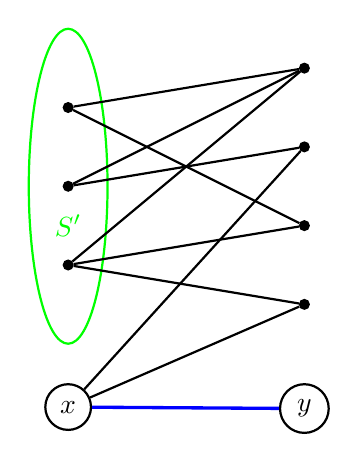
\begin{tikzpicture}[
  dot/.style = {
    shape = circle,
    fill = black,
    minimum size = 4pt,
    inner sep = 0pt,
    outer sep = 0pt,
  },
  every path/.style = {
    thick
  }
]
  \draw[color = green] (0, 2) ellipse (0.5cm and 2cm);
  \draw[color = green] node at (0, 1.5) {\(S'\)};

  \draw node[dot] (L1) at (0, 3) {};
  \draw node[dot] (L2) at (0, 2) {};
  \draw node[dot] (L3) at (0, 1) {};
  \draw node[below, circle, draw = black] (L4) at (0, -0.5) {\(x\)};

  \draw node[dot] (R1) at (3, 3.5) {};
  \draw node[dot] (R2) at (3, 2.5) {};
  \draw node[dot] (R3) at (3, 1.5) {};
  \draw node[dot] (R4) at (3, 0.5) {};
  \draw node[below, circle, draw = black] (R5) at (3, -0.5) {\(y\)};

  \draw (L1) edge (R1) edge (R3);
  \draw (L2) edge (R1) edge (R2);
  \draw (L3) edge (R1) edge (R3) edge (R4);
  \draw (L4) edge (R2) edge (R4);
  \draw[very thick, color = blue] (L4) -- (R5);
\end{tikzpicture}

    \caption{1ый случай (a)}\label{fig:hall-case-1-a}

  \end{subfigure}
  \qquad
  \begin{subfigure}[b]{0.3\textwidth}

    \centering
    \input{figures/GT/07/case_01_b.tex}
    \caption{1ый случай (b)}\label{fig:hall-case-1-b}

  \end{subfigure}
  \qquad
  \begin{subfigure}[b]{0.3\textwidth}

    \centering
    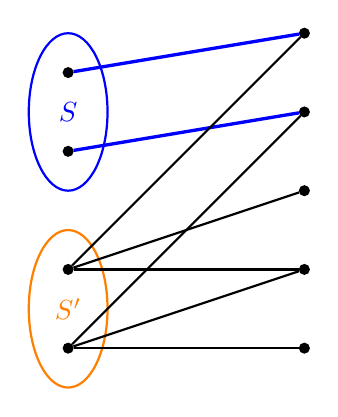
\begin{tikzpicture}[
  dot/.style = {
    shape = circle,
    fill = black,
    minimum size = 4pt,
    inner sep = 0pt,
    outer sep = 0pt,
  },
  every path/.style = {
    thick
  }
]
  \draw[color = blue] (0, 2.5) ellipse (0.5cm and 1cm);
  \draw[color = blue] node at (0, 2.5) {\(S\)};

  \draw[color = orange] (0, 0) ellipse (0.5cm and 1cm);
  \draw[color = orange] node at (0, 0) {\(S'\)};

  \draw node[dot] (L1) at (0, 3) {};
  \draw node[dot] (L2) at (0, 2) {};
  \draw node[dot] (L3) at (0, 0.5) {};
  \draw node[dot] (L4) at (0, -0.5) {};

  \draw node[dot] (R1) at (3, 3.5) {};
  \draw node[dot] (R2) at (3, 2.5) {};
  \draw node[dot] (R3) at (3, 1.5) {};
  \draw node[dot] (R4) at (3, 0.5) {};
  \draw node[dot] (R5) at (3, -0.5) {};

  \draw[very thick, color = blue] (L1) -- (R1);
  \draw[very thick, color = blue] (L2) -- (R2);
  \draw (L3) edge (R1) edge (R3) edge (R4);
  \draw (L4) edge (R2) edge (R4) edge (R5);
\end{tikzpicture}

    \caption{2ой случай}\label{fig:hall-case-2}

  \end{subfigure}
\end{figure}

\begin{proof}
  \(\implies\) Если в графе существует \(X\)-совершенное паросочетание, то для
  любого \(x \in X\) существует уникальный сосед в \(Y\), значит количество
  соседей у любого \(S \subseteq X\) будет как минимум \(\abs{x}\).

  \(\impliedby\) Индукция по \(\abs{X}\).

  \textbf{База}: \(\abs{X} = 1\). Очевидно, что \(X\)-совершенное паросочетание
  существует тогда и только тогда, когда у единственной вершине в \(X\) будет
  как минимум один сосед из \(Y\).

  \textbf{Переход}: пусть теорема верна при \(\abs{X} < n\). Рассмотрим граф,
  удовлетворяющий условиям теоремы, в котором \(\abs{X} = n\). Возможны два
  случая:

  \begin{enumerate}
    \item \(\forall S \subseteq X \colon \abs{N(S)} > \abs{S}\)

    Выберем произвольный \(x \in S\) и поставим ему в пару любого из его
    соседей. Обозначим этого соседа \(y\), а оставшиеся в \(S\) вершины \(S'\).

    Т.к. до выбора соседа для \(x\) выполнялось неравенство
    \(\abs{N(S')} > \abs{S'}\), то после выбора соседа выполняется неравенство
    \(\abs{N(S')} \ge \abs{S'}\), т.к. количество свободных соседей \(S'\) могло
    уменьшиться не более чем на один (оно уменьшилось на один в случае, если
    \(y \in N(S')\)).

    Пары для оставшихся вершин мы можем найти по предположению индукции.

    \item \(\exists S \subseteq X \colon \abs{N(S)} = \abs{S}\)
    
    Каждому \(x \in S\) по предположению индукции поставим в пару одного из его
    соседей. Рассмотрим оставшиеся вершины \(S' = X \setminus S\). Покажем, что
    для них тоже можно найти пару.

    Пусть найдется такое \(P \subseteq S'\), что \(\abs{N(P)} < \abs{P}\). Тогда
    рассмотрим множество \(S \cup P\). Т.к. \(\abs{N(S)} = \abs{S}\) и
    \(\abs{N(P)} < \abs{P}\), то \(\abs{N(S \cup P)} < \abs{S \cup P}\). Это
    противоречит условию теоремы, значит
    \(\forall P \subseteq S' \colon \abs{N(P)} \ge \abs{P}\), поэтому по
    предположению индукции мы можем найти пары для всех \(x \in S'\).
  \end{enumerate}
\end{proof}
